\documentclass[12pt]{article}

% House style preamble: central symlink only.
\input{.house-style/preamble.tex}

% --- Anonymization toggle for double-blind review ---
\newif\ifblind
\ifdefined\blindbuild \blindtrue \else \blindfalse \fi

\hypersetup{
  pdftitle={Production probability, transport, and grammatical possibility: Reanalysing the English dative alternation with open data},
  pdfkeywords={dative alternation, production probability, transport, projectibility, grammaticality, corpus linguistics, acceptability}
}
\ifblind\hypersetup{pdfauthor={}}\fi

\title{Production probability, transport, and grammatical possibility\\
{\large Reanalysing the English dative alternation with open data}}
\ifblind
  \author{[Author name, Open Researcher and Contributor ID (ORCID), and affiliation removed for double-blind review]}
\else
  \author{Brett Reynolds \orcidlink{0000-0003-0073-7195}%
  \thanks{Contact: \href{mailto:brett.reynolds@humber.ca}{brett.reynolds@humber.ca}}\\
  Humber Polytechnic \& University of Toronto}
\fi
\date{June 2026}

\begin{document}
\maketitle

\begin{abstract}
This paper develops a no-new-data reassessment of \textcite{bresnan2007}. The
current analyses reproduce the production-choice target from
\texttt{languageR::dative}, add explicit null and partial-pooling checks, and
test whether the resulting conditioning profile transports to the Spoken
British National Corpus 2014 (BNC2014) dative dataset. It then adds a compact
DAIS acceptability bridge for the same high-frequency verb core. The
result is that modern modelling preserves the classic production conclusion;
within the shared high-frequency verb set, source-trained structural predictors
retain substantial same-row discrimination in BNC2014, while target-native
out-of-fold predictions reveal local calibration and residual lexical
structure. DAIS preferences show moderate marginal correspondence with the
production scores but are systematically more favourable to the double-object
alternative, and the production score adds little once the experimental
conditions are represented directly. The paper reads these results through
projectibility: production probability, acceptability preference, and
grammatical possibility are related evidence channels, not one repeated
measurement.
\end{abstract}

\noindent\textbf{Keywords:} dative alternation; production probability; transport; projectibility; grammaticality; corpus linguistics; acceptability

\section{The problem}

A corpus-based probabilistic grammar can predict held-out observations from its
own source corpus and still fail when it's moved to another corpus. External
validation needs more than a single discrimination statistic. It needs
probability scoring, calibration, comparison with target-native predictions on
the same observations, an account of which predictors carry the transport, and a
specification of the opportunity set over which the predictions are defined. This
paper assembles that regime and runs it on a canonical case. Throughout,
\term{probabilistic grammar} names the fitted production model, not a claim
about speakers' competence or a community's licensing of forms; external
validation bears on the model's predictive transport, not directly on either.

The English dative alternation is that case. Speakers can say \mention{give Kim
the book} or \mention{give the book to Kim}, and the choice is uneven: it varies
with verb, length, animacy, definiteness, pronominality, discourse status,
corpus, and register. The unevenness is easy to misread, because a rare pattern
can be lexically restricted, strongly dispreferred, or tied to a discourse
context without falling outside the grammar. \textcite{bresnan2007} modelled that
conditioning and argued that corpus probabilities can reveal grammatical
possibilities informal judgements miss.

The model has since been shown to travel: trained on one variety and scored on
another, it keeps much of its accuracy
\citep{BresnanHay2008,KendallBresnanVanHerk2011,EngelEtAl2025}. The open question
isn't whether it travels but how well, once transport is treated as a full
predictive-evaluation problem, and what a fitted production probability can and
can't say about grammar. That last is a question of \term{projectibility}, what
observing a profile in one setting licenses about another \citep{Goodman1955}.

The argument proceeds by separating validation claims that are often collapsed.
Reproducing the source model asks whether the classic production profile is
stable in its original data. Scoring frozen predictions in BNC2014 asks whether
that profile carries predictive information out of domain. Comparing those
predictions with a target-native model on the same rows asks how much local
structure the source model misses. Calibration and ablation then ask whether the
transport is a matter of ranking, probability level, lexical base rates, or
non-lexical conditioning. Finally, an acceptability bridge asks where a
production probability is licensed, and where it isn't, when carried into a
judgement channel.

\section{The original target}

\textcite{bresnan2007} is the anchor because it treats the alternation as a
grammatical problem, not a simple frequency count: the claim isn't that
whatever occurs often is grammatical, but that observed choices expose
systematic constraints on what speakers treat as available. That matters because
informal judgements compress several diagnostics into one feeling. A
construction may sound odd because no viable analysis is available, because a
verb--construction pairing conflicts with an established value, because the
relevant discourse or communicative situation is missing, because speakers have
too little evidence to settle a rare form's status, because an established
competitor keeps winning where the form might otherwise appear, or because
processing pressure makes a recoverable structure feel bad. Corpus data,
especially when normalized to the relevant opportunity set and paired with
judgement evidence, can help sort these cases.

The empirical target is production choice. In Bresnan et al.'s data the response
is whether the recipient appears as a noun phrase (NP), in the double-object
pattern, or as a prepositional phrase (PP), in the prepositional dative, with
predictors for the verb, recipient, theme, discourse status, and corpus. This
paper preserves that target and treats the production probability as evidence to
interpret, not as a direct measure of grammaticality.

\section{Data and direct replication}

This section will report the verified \texttt{languageR::dative} data path and
the direct production-choice target. The initial inspection confirms 3,263 rows,
15 columns, and the NP/PP outcome used for the first reproducible reanalysis.
The baseline analysis should be presented as a disciplined reproduction step,
not as the paper's final contribution.

\section{Modern modelling update}

This section will report the baseline, null, and partial-pooling results. The
important finding is conservative: the hierarchical verb-intercept model
essentially matches the fixed-verb model and preserves Bresnan et al.'s
production-choice conclusion. Modern modelling changes the statistical
packaging more than the linguistic conclusion.

\section{Generalization and acceptability}

The BNC2014 analysis asks whether the production profile travels across corpus
design, variety, period, and annotation regime. The transport model is trained
on the spoken \texttt{languageR} rows restricted to the six BNC2014 verbs. It's
then evaluated on harmonized BNC2014 rows, with complete-case filtering stated
as part of the evidential scope.

Three estimands are kept apart. The \texttt{languageR} models estimate
conditional production choice among attested noun phrase and prepositional
phrase dative tokens. The BNC2014 transport result estimates out-of-domain
predictive performance over complete-case rows in the six shared
high-frequency verbs after harmonization. DAIS estimates controlled
double-object preference for constructed alternatives. These numbers can
therefore be read together only as different evidence channels, not as repeated
measurements of one quantity.

Cross-variety probabilistic grammar of the dative isn't new ground.
\textcite{BresnanFord2010} compared American and Australian English and found
that speakers' probabilistic choice knowledge is largely shared across
varieties, but varies enough to surface in naturalness ratings and
lexical-decision latencies. \textcite{RothlisbergerGrafmillerSzmrecsanyi2017}
extended the comparison across nine post-colonial Englishes and found broad
stability with local traces of indigenization. So the bare finding that dative
conditioning largely travels wouldn't, on its own, be new.

Two things here are different. First, it's a strict out-of-domain test: one
model is fit on one corpus and scored on another against held-out log loss, area
under the curve, and scrambled-label nulls, rather than fit separately within
each variety. Second, the transport result feeds a distinction the variationist
work doesn't draw, between production probability and grammatical possibility,
developed in the next section. The contribution is that framing and the test, not
the stability itself.

The comparison is therefore an out-of-domain transport test. The first
transport model holds modality close by training only on spoken
\texttt{languageR} rows, but the corpus shift is still large: American
telephone conversation from 1990--1991 to spontaneous British conversation from
2012--2014, under a different annotation scheme and a six-verb target set.
That target set is already a scope restriction. In \texttt{languageR}, those six
verbs account for 2,201 of 3,263 rows, and for 1,564 of 2,360 spoken rows. They
are the high-frequency core, not a random sample of the alternation.

Harmonization is lossy. The outcome maps cleanly: \texttt{VNN} becomes NP and
\texttt{VNPP} becomes PP. Verb also maps cleanly after restricting the
\texttt{languageR} data to the six shared verbs. Length needs more care. The
released BNC2014 length fields are character counts: the data dictionary defines
\texttt{RecLen} and \texttt{ThemeLen} as the number of characters in the
recipient and theme \citep{JensetMcGillivray2019Dative}. Those aren't comparable
to \texttt{languageR}'s token-like lengths, so the released fields can't enter
the transport model directly. The script instead derives word counts from the
recipient and theme strings. Two costs follow: the whitespace tokenization isn't
guaranteed to match the convention behind \texttt{languageR}'s counts, and the
few rows with empty phrase strings drop out, since a character count can't be
turned back into a word count.

Several predictors are available only as proxies. BNC2014 has recipient and
theme animacy, theme definiteness, and recipient/theme pronominality, but some
fields have missing values and different annotation paths. Recipient
definiteness is not released as a field, so it enters only as a labelled regex
proxy in a sensitivity check. Discourse accessibility is unavailable and is
dropped from transport.

The core transport model therefore scores the 1,621 BNC2014 rows complete for
the harmonized predictors, not all 1,839 released dative rows. The missing rows
are not neutral: noun phrase recipients make up 0.819 of the complete rows but
only 0.670 of the 218 incomplete rows. The headline comparison is consequently
a complete-case estimate over the shared high-frequency core.

A BNC2014 metadata audit makes the domain label concrete. In the released
dative rows, Level 1 dialect is \enquote{uk} for 1,720 of 1,839 rows and Level 2
dialect is \enquote{english} for 1,689. Gender is female-coded for 1,138 rows
and male-coded for 699, and the largest age band is 19--29 with 736 rows.
Interaction type is also skewed: close-family, partner, and very-close-friend
conversations contribute 1,171 rows, while friends and wider-family
conversations contribute another 538. The complete-case subset has the same
shape. A single BNC2014 transport score should therefore be read as a
corpus-domain diagnostic, not as a clean estimate for British spoken English in
general.

\begin{table}[htbp]
\centering
\small
\begin{tabular}{>{\raggedright\arraybackslash}p{0.48\linewidth}>{\raggedright\arraybackslash}p{0.22\linewidth}rr}
\toprule
Model & Test data & Log loss & AUC \\
\midrule
\texttt{languageR} marginal & BNC2014 complete & 0.473 & 0.500 \\
\texttt{languageR} core transport & BNC2014 complete & 0.308 & 0.906 \\
\texttt{languageR} core transport & Scrambled BNC2014 complete & 0.885 & 0.515 \\
BNC2014 marginal holdout & BNC2014 complete & 0.481 & 0.500 \\
BNC2014 native core holdout & BNC2014 complete & 0.202 & 0.960 \\
BNC2014 native scrambled train & BNC2014 complete & 0.495 & 0.440 \\
\bottomrule
\end{tabular}
\caption{First BNC2014 complete-case transport and native holdout comparisons.}
\label{tab:bnc-transport}
\end{table}

The transported core model beats the marginal baseline by a wide margin. Its
test log loss is 0.308, compared with 0.473 for the \texttt{languageR} marginal
baseline, and its AUC is 0.906. A percentile bootstrap over the BNC2014
complete-case test rows (2,000 resamples) puts the log loss in [0.277, 0.337]
and the AUC in [0.890, 0.922], so the result isn't an artefact of one lucky
split. When the BNC2014 outcome is scrambled, the same predictions collapse to
0.885 log loss and 0.515 AUC.

Simple all-row imputation checks make the complete-case scope visible. With
missing lengths set to their BNC2014 medians and missing binary predictors set
to their modes, the transported model scores 0.362 log loss and 0.872 AUC on all
1,839 rows. Filling the missing binary predictors uniformly as \enquote{no} or
\enquote{yes} gives 0.312/0.911 and 0.408/0.856, respectively. The direction of
the transport result survives, but the exact headline strength is sensitive to
the missingness treatment.

Raw accuracy is a weak lens here. The recipient is an NP in about four of five
complete-case BNC2014 tokens, so a majority-class baseline already scores near
0.82, and the transported model reaches only about 0.86. The gain that matters
shows up in discrimination and calibration, the AUC of 0.906 and the lower log
loss, not in the accuracy headline.

\begin{figure}[htbp]
\centering
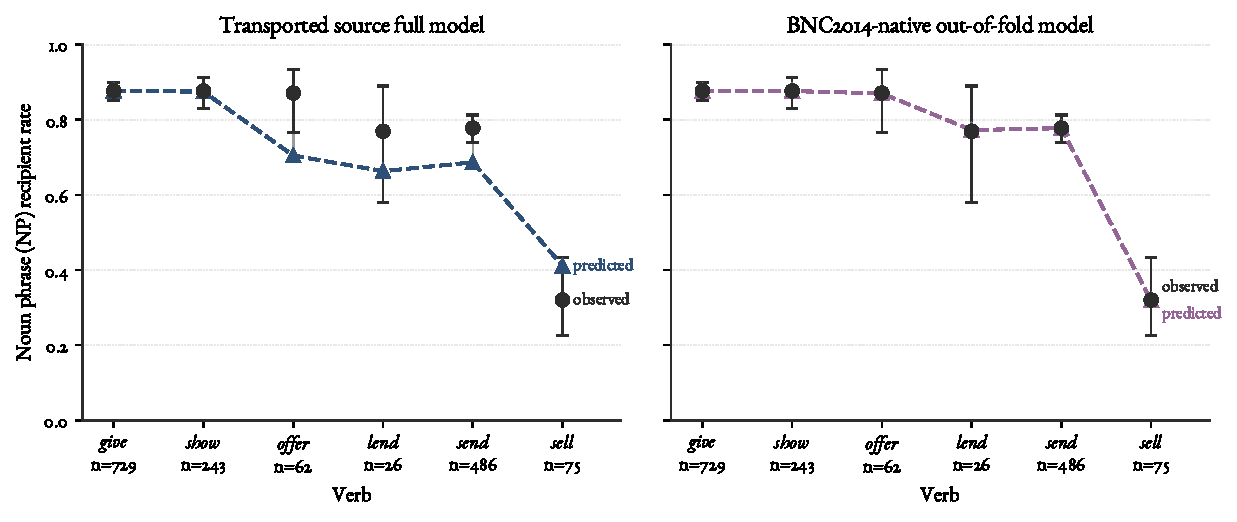
\includegraphics[width=\linewidth]{data/derived/figures/bnc2014_transport_calibration_by_verb.pdf}
\caption{Verb-level calibration for the transported \texttt{languageR} model
and the BNC2014-native holdout model. The vertical axis is the noun phrase
(NP) recipient rate. Sample sizes are shown under each verb.}
\label{fig:bnc-calibration}
\end{figure}

That framing changes the interpretation of the result. Success is evidence that
the conditioning profile is projectible across the bundled corpus shift within
the shared high-frequency core, not just refittable. Failure, if it had
occurred, would not have identified a single cause: variety, date, register,
verb restriction, and annotation all move together.

A scope limit bounds how far this generalizes. The six shared verbs are among
the most frequent and canonical members of the alternation, so transport is
tested where the conditioning profile is most likely to hold. The two datasets
intersect only on this high-frequency core; verbs with marginal, contested, or
idiosyncratic dative behaviour aren't shared, so they go untested here. The
result therefore licenses a claim about the core, not about the periphery, where
projectibility is hardest to establish.

The BNC2014-native model is still stronger. On a verb-stratified BNC2014
holdout split, the native core model reaches 0.202 log loss (bootstrap
[0.154, 0.254]) and 0.960 AUC (bootstrap [0.938, 0.979]). The gap is not small:
the transported model's log loss is about half again the native model's, and the
two bootstrap intervals don't overlap on either metric, so the difference isn't
just split noise. The transported model has learned a useful profile, but
BNC2014 also contains local structure that the \texttt{languageR} fit doesn't
capture.

Read the gap as a bounded downgrade rather than an apology. The transported
model clears the marginal and scrambled-label comparisons, so the result is not
just a same-corpus artefact. But the residual gap cannot be assigned to variety,
period, register, annotation, or the six-verb restriction one by one. Those
dimensions are bundled in this comparison.

Several directions travel. Recipient length is negative for NP realization;
theme length is positive; recipient pronominality is strongly positive; theme
pronominality is strongly negative; \texttt{sell} and \texttt{send} are less
NP-like than \texttt{give}. These are the strongest signs that the Bresnan
profile is projectible beyond one packaged dataset.

Some details do not travel cleanly. The transported model underpredicts NP
realization for \texttt{send}, \texttt{offer}, and \texttt{lend}, and
overpredicts it for \texttt{sell}. Theme definiteness is the clearest
coefficient mismatch: negative in the \texttt{languageR}-trained model, positive
and weak in the BNC2014-native model.

The recipient-definiteness proxy should stay a sensitivity check. Adding it
worsens transport log loss from 0.308 to 0.347 while leaving AUC essentially
unchanged. That pattern fits the harmonization note: the proxy is interpretable,
but it should not carry the headline result.

Acceptability evidence answers a different question. The Dative Alternation and
Information Structure (DAIS) dataset, introduced by
\textcite{HawkinsYamakoshiGriffithsGoldberg2020VerbBias}, contains 50,000 human
judgements over 5,000 dative sentence pairs and systematically varies verb,
definiteness, and argument length. The repository now carries a CC BY 4.0
licence, and the dataset authors have given explicit permission to reuse the
judgements. DAIS can therefore enter as a compact bridge
\citep{HawkinsYamakoshiGriffithsGoldberg2020DAIS}.

The bridge keeps the targets separate. I score only the 150 DAIS items whose
verbs overlap the six-verb production core. The same spoken \texttt{languageR}
production model that was transported to BNC2014 predicts a noun-phrase
recipient probability for each constructed DAIS pair; the DAIS item mean gives
the corresponding human double-object preference on a 0--1 scale. As a bridge
analysis, it asks whether a production probability profile and a controlled
preference profile point in the same direction.

\begin{figure}[htbp]
\centering
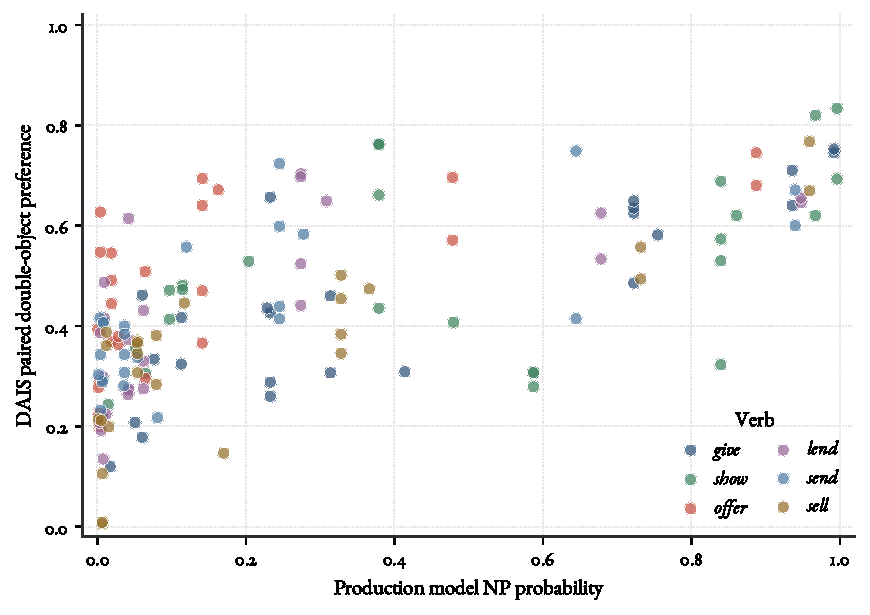
\includegraphics[width=0.82\linewidth]{data/derived/figures/dais_production_preference_bridge.pdf}
\caption{DAIS production/preference bridge for the six shared verbs. Each point
is a constructed DAIS item. The horizontal axis is the spoken
\texttt{languageR} model's noun phrase (NP) recipient probability; the vertical
axis is DAIS double-object (DO) preference. The diagonal marks equality between
the two channels, and the \mention{offer} cluster is highlighted because it
shows the clearest channel separation.}
\label{fig:dais-bridge}
\end{figure}

\begin{table}[htbp]
\centering
\small
\begin{tabular}{lrrr}
\toprule
Verb & Prod. NP prob. & DAIS DO pref. & Difference \\
\midrule
\mention{give} & 0.408 & 0.449 & -0.041 \\
\mention{lend} & 0.204 & 0.426 & -0.222 \\
\mention{offer} & 0.150 & 0.468 & -0.319 \\
\mention{sell} & 0.231 & 0.351 & -0.120 \\
\mention{send} & 0.196 & 0.428 & -0.232 \\
\mention{show} & 0.506 & 0.516 & -0.009 \\
\bottomrule
\end{tabular}
\caption{DAIS bridge for the six shared verbs. The DAIS column is the item-level
mean double-object (DO) preference. The production column is the noun-phrase
(NP) recipient probability from the spoken \texttt{languageR} core model.}
\label{tab:dais-bridge}
\end{table}

The two channels line up moderately, while remaining distinct. With
\mention{something} treated as a pronominal theme, Pearson's \(r\) is 0.667 and
Spearman's \(\rho\) is 0.685 over the 150 shared-verb items. The mean production
NP probability is 0.283, while the mean human DO preference is 0.440. Treating
\mention{something} as nonpronominal gives the same interpretation
(\(r = 0.645\), \(\rho = 0.675\), mean production probability 0.343).
The participant-level check points the same way without making the correlation
carry the whole inference. A mixed model on 1,525 shared-verb judgements from
923 participants, with random intercepts for participant and verb, is
non-singular; once recipient condition and theme type are included, the
incremental production-score coefficient is small (0.052, standard error
0.060). The bridge is therefore evidence of shared conditioning and diagnostic
divergence, not validation of one channel by the other.

The useful cases are the divergences. \mention{Offer} is the clearest verb-level
one: the production model makes it strongly PP-like, but DAIS participants are
much more willing to choose the double-object version. For example,
\enquote{Juan offered the woman a payment} has predicted NP probability 0.141
but DAIS DO preference 0.694. The point is channel separation: judgement
preference can occupy a different region of the evidence space from corpus
production probability.

\section{Grammatical possibility}

The empirical result supports a sharper vocabulary, not a shortcut from
frequency to grammar. The \texttt{languageR} analysis shows that a classic
production profile is reproducible under explicit validation. The BNC2014
analysis shows that much of that profile travels to a later spoken British
corpus. Both results concern production choice.

The target is grammaticality, a contested construct that I'll take as a
community-conditioned licensing status for form--value, or form--meaning,
relations \citep{pullum2019-normativity,nefdt2023}. Cognitive and social
mechanisms stabilize that status across a speech community. The status is
graded, not a clean threshold: a form belongs to the grammar to the degree that
the relevant relation is licensed strongly enough to project to new cases,
including cases that are rare, strongly conditioned, or absent from a finite
corpus. That projection is the point. A category earns its keep by being
projectible for a purpose \citep{Goodman1955,boyd1999}, and the purpose here is
predicting realization in unseen contexts and telling rare-but-grammatical cases
apart from ungrammatical ones.

Acceptability preference, raw judgement, corpus frequency, formal generability,
and standardness are neighbouring constructs. They can bear on licensing, but
none fixes it alone. A corpus token records what a speaker or writer did in a
context. A judgement task samples a noisy, role-dependent instrument: how a
speaker, participant, or evaluator responds to constructed alternatives under
controlled conditions.

The useful distinction is between target and channel. Corpus choices are one
channel: they show which form was realized when an alternation token occurred.
Judgements are another channel: they provide detector responses calibrated to a
speech community and task role. Grammaticality is the target those channels bear
on indirectly.

Everything here is conditioned on the opportunity set. This corpus evidence
covers attested dative-alternation tokens: cases already annotated as NP or PP
recipient realizations. It can support claims about which realization speakers
chose inside that frame. A broader corpus design could estimate other
opportunities: transfer events expressed by non-dative paraphrase, left implicit
in context, or paired with an independent acceptability task. These released
rows don't provide that broader denominator.

\begin{figure}[htbp]
\centering
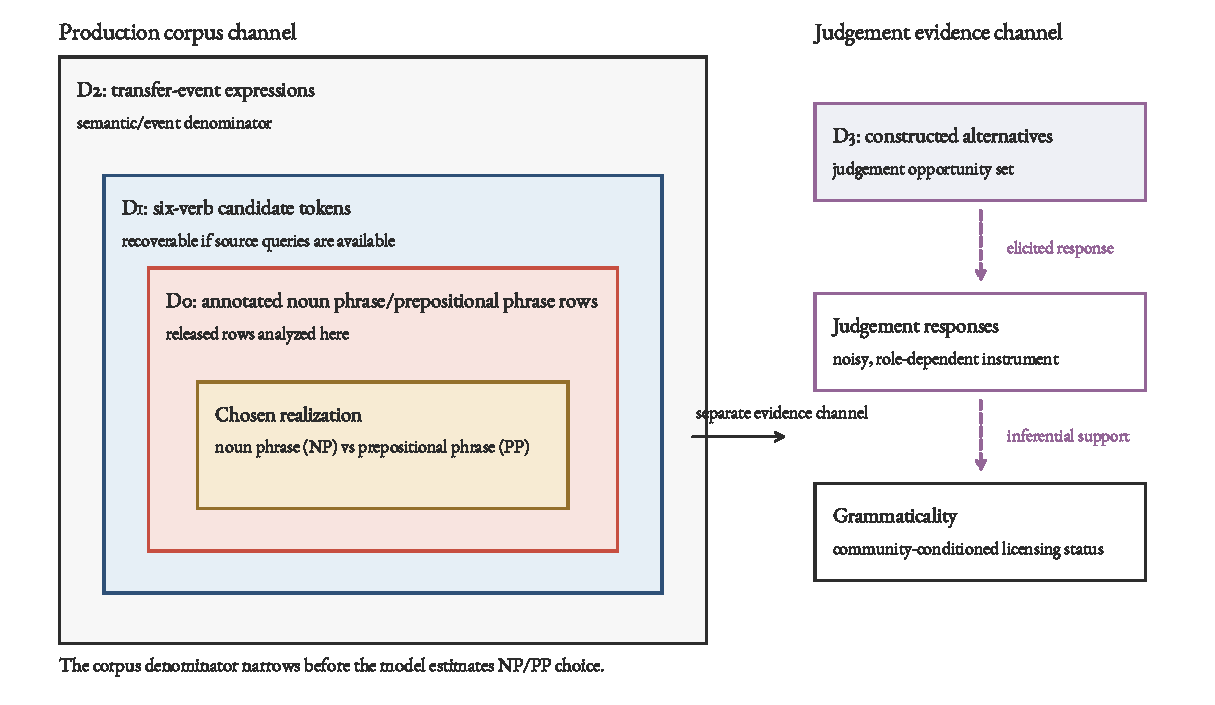
\includegraphics[width=\linewidth]{data/derived/figures/opportunity_sets_nested.pdf}
\caption{Nested opportunity sets for the dative-alternation evidence. The
released corpus rows estimate realization choice inside the annotated noun
phrase/prepositional phrase denominator. Broader transfer-event and judgement
opportunity sets would answer different questions about grammaticality.}
\label{fig:opportunity-sets}
\end{figure}

Production data can support claims about grammaticality only through an
explicit bridge from attested choices to possible alternatives. Figure
\ref{fig:opportunity-sets} marks where that bridge would have to be built.

The dative alternation makes the bridge visible. A low-probability double-object
realization may be grammatical but dispreferred under the observed predictors.
A prepositional realization may be likely because the theme is short and the
recipient is long. A form may be absent because the corpus lacks the relevant
verb, register, or discourse setting.

No amount of additional production data closes this gap. A production model
estimates choice among realizations that occurred, and it's silent by
construction about realizations that are grammatical but unattested, or
grammatical outside the sampled frame. More tokens enlarge the attested region
without ever reaching the unattested-but-grammatical one. The boundary between
production probability and grammatical possibility isn't a defect of
\texttt{languageR::dative} or BNC2014; it's a general constraint on what usage
frequency can show about grammar.

In one sense this restates a familiar point: performance data underdetermine
competence, and no finite corpus fixes the grammar
\citep{chomsky1965,Miller1963}. What the dative case adds is a measurable,
channel-specific version of that boundary. The opportunity set says which cells
a production channel can and can't reach, so the gap stops being a slogan and
becomes a property of a stated dataset and design, open to the same kind of
modelling the rest of the paper uses.

The current analyses therefore license a cautious claim. Bresnan et al.'s
production-conditioning profile is durable and partly transportable. That
supports the idea that corpus probabilities can reveal structure that informal
judgements miss. It does not make production probability identical to
grammaticality. What the durable, transportable profile does buy is prediction:
it forecasts realization for unseen tokens within its scope of verbs, registers,
and varieties, and it marks the low-probability cells where grammaticality has to
be settled through another channel.

\section{Conclusion}

TODO: Conclude with the methodological lesson, not the dataset. The project
should show how a classic corpus-probabilistic result can be made reproducible,
portable, and conceptually useful for the ontology of grammatical possibility.


\section*{Data and code availability}

The public working repository is
\href{https://github.com/BrettRey/bresnan-dative-alternation-reanalysis}{\texttt{BrettRey/bresnan-dative-alternation-reanalysis}}.
A submission release should archive the exact commit or digital object
identifier. The analysis scripts fetch public datasets to temporary locations
and validate downloaded files by checksum.

\begin{center}
\small
\begin{tabular}{ll}
\toprule
File & MD5 \\
\midrule
BNC2014 CSV & \texttt{1c041dbcb635855f3d8f4be9f3e1fced} \\
DAIS item CSV & \texttt{46af310f1633b8784f897e4482faed84} \\
DAIS cleaned-judgement ZIP & \texttt{e7b3ac6f2dd8e85bc93e6e20fc0f6ec1} \\
\bottomrule
\end{tabular}
\end{center}

Derived files and the source-verification note are stored in the repository;
the README gives their paths. The principal reproduction commands are:

\begin{quote}
\small
\texttt{Rscript analysis/08\_dais\_acceptability\_bridge.R}\\
\texttt{Rscript analysis/09\_bnc2014\_metadata\_scope.R}\\
\texttt{Rscript analysis/10\_bnc2014\_paired\_transport\_cv.R}\\
\texttt{python3 analysis/06\_denominator\_and\_figure\_candidates.py}\\
\texttt{make}
\end{quote}

The cross-validation and bootstrap seed is \texttt{20260625}. Session
information is written to a derived text file. Raw DAIS files aren't committed.

\section*{Acknowledgements}

Drafting, coding, and review used Codex/GPT 5.5 and Claude
Opus 4.8. All analysis decisions, source checks, and final text remain the
author's responsibility.

\clearpage
\printbibliography

\end{document}
